\documentclass[a4paper,11.5pt]{article}
\usepackage[latin1]{inputenc}
\usepackage[T1]{fontenc}
\usepackage[english]{babel}
\usepackage{graphicx}
\usepackage{amsmath}
\usepackage{amsfonts}
\usepackage{multirow}
\usepackage{booktabs}
\usepackage{bbold}
\usepackage{mathtools}
\usepackage{mathrsfs}
\usepackage{enumitem}
\usepackage{array}
\usepackage{float}

\setlength{\parindent}{0pt}
\DeclarePairedDelimiter{\floor}{\lfloor}{\rfloor}
\DeclarePairedDelimiter{\ceil}{\lceil}{\rceil}

\newcommand{\vt}{\boldsymbol}

\title{Digital Communications - HW3}
\author{Jacopo Pegoraro, Edoardo Vanin}
\date{21/05/2018}

\begin{document}

\maketitle

We have to implement six different versions of the receiver structure in a QPSK modulation scheme. First we present the setup of the transmitter and the channel as given, then we analyze the different configurations one by one and give a brief discussions of the resulting probabilities of symbol error obtained from simulation over different values of the SNR at the channel output, $\Gamma$. 

\section*{Transmitter and Channel}

The system takes a sequence of input symbols $a_k$ at sampling time $T=1$ and applies an upsampling of factor 4, obtaining $a_k'$ at $T/4$. This new sequence is then filtered by $q_c$ as described by the following difference equation:
\begin{equation}
s_c(nT/4) = 0.67 s_c((n-1)T/4) + 0.7424 a_{n-5}
\end{equation}
After the filtering white noise is added. The SNR at the channel output for all the configurations in this first phase is $\Gamma = 10$ dB, so from the following relations we can derive $\sigma_w^2$, the variance of the complex valued Gaussian noise:
\begin{equation}
\Gamma = \frac{M_{s_c}}{N_0\frac{1}{T}} = \frac{\sigma_a^2 E_{q_c}}{\sigma_w^2} \longrightarrow \sigma_w^2 = \frac{\sigma_a^2 E_{q_c}}{\Gamma} = 2\sigma_I^2
\end{equation}
where $\sigma_I^2$ is the variance per component. In addition we can also compute the PSD as $N_0=\sigma_w^2 T_c=\sigma_w^2/4$, because the sampling time $T_c$ at which we add the noise is $T/4$.
In figure \ref{fig:qc} we plot the impulse response and the frequency response of the filter $q_c$.
This implementation of the transmitter is the same for all the following discussion.

\begin{figure}[H]
	\begin{center}   
		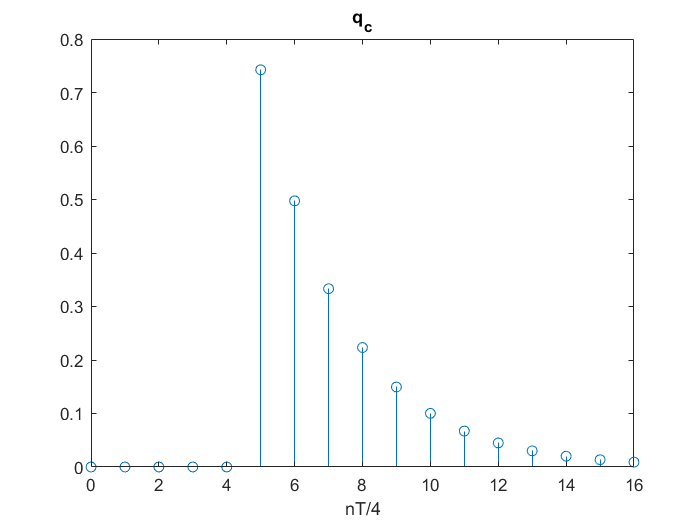
\includegraphics[width=\textwidth]{figs/q_c.png} 
		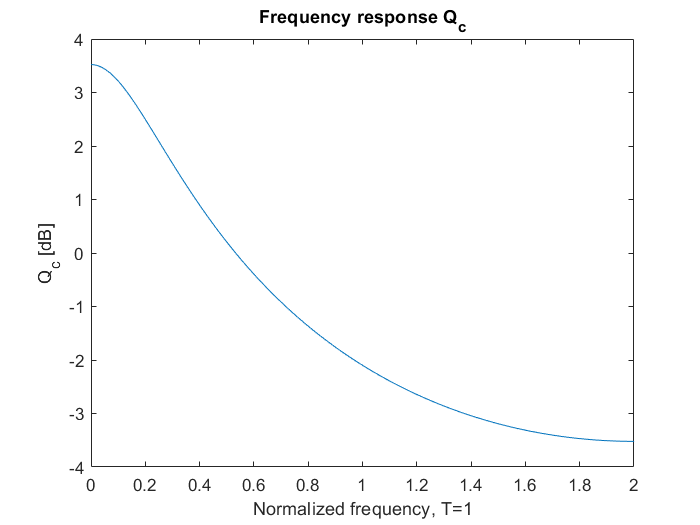
\includegraphics[width=\textwidth]{figs/Qc.png} 
		\caption{Impulse and frequency response of the filter $q_c$ at $T/4$.}
		\label{fig:qc}
	\end{center}
\end{figure} 

\section*{Point A}

In point A at the receiver we have a matched filter $g_{M}$ (see figure \ref{fig:A_gm}), obtained from $q_c$ as $g_M=q_c^*(t_0-t)$. For simplicity in the last formula we have denoted the filters as is they were defined on continuous time while in the actual simulation they are at $T/4$. 

\begin{figure}[H]
	\begin{center}   
		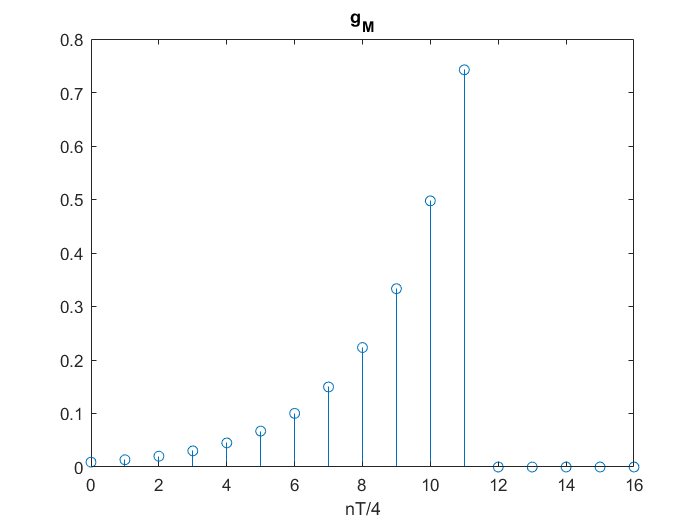
\includegraphics[width=\textwidth]{figs/A_gm.png} 
		\caption{Impulse response of the matched filter $g_{M}$ for the receiver in point A.}
		\label{fig:A_gm}
	\end{center}
\end{figure} 

The output of the matched filter is then sampled at $T$ starting from an initial offset called \emph{timing phase} $t_0$. In our case the choice of $t_0$ is made easy by the presence of the matched filter, as we can just choose the value $\bar{t}_0$, multiple of $T/4$, that is the index of the peak of the correlation between $q_c$ and $g_M$, then $t_0$ will be equal to $\bar{t}_0 T/4$. Following this reasoning we chose $\bar{t}_0=16$ (17 with Matlab indexing), equal also to the index of the last sample of $g_M$ (see figure \ref{fig:A_gm}).

The signal is then passed to a linear equalizer (LE) derived by a particular case of a Decision Feedback Equalizer (DFE) where we only have the feedforward filter $c$ (see point B for the detailed analysis of the DFE). The signal at this point in the receiver system is called $x_k$ and is the result of the convolution of the input sequence $a_k$ with the overall impulse response $h_i = q_c * g_M$ that goes from $-N_1$ to $N_2$. We will call precursors the taps of $h$ that go from $-N1$ to $-1$ and postcursors the taps from $1$ to $N_2$. To obtain the coefficients of $c$ we used the Wiener approach on the input random process and solved the Wiener-Hopf equation $\vt{c}_{opt}=\vt{R}^{-1}\vt{p}$ using the matrix $\vt{R}$ and vector $\vt{p}$ as in equations \ref{eq:wienerR} and \ref{eq:wienerp} with the parameter $M_2$ (the order of the feedback filter) set to $0$ because we have no feedback filter in this case. The free parameters that we have to choose are $M_1$, the order of filter $c$ and $D$ the delay that it will introduce on the input sequence. We carried out this choice looking at the value of the cost function $J_{min}$ (see equation \ref{eq:jmin}) for each combination of the two parameters, preferring low values if possible to avoid increasing the complexity. The best choice in this case was $M_1=5$ and $D=2$.
In figure \ref{fig:A_c} we plot the impulse response $c_i$ at sampling time $T$ as obtained from the Wiener solution. 

\begin{figure}[H]
	\begin{center}   
		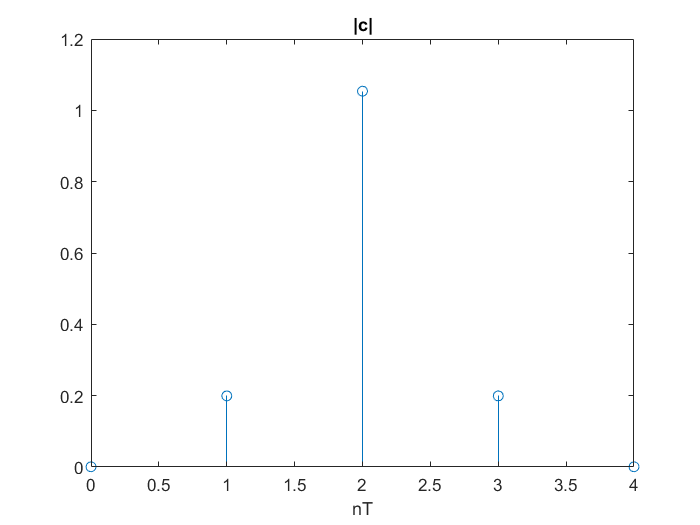
\includegraphics[width=\textwidth]{figs/A_c.png} 
		\caption{Magnitude of the impulse response of filter $c$ in point A.}
		\label{fig:A_c}
	\end{center}
\end{figure}

The aim of filtering with $c$ is to obtain an overall impulse response of the system that satisfies the Nyquist conditions for the absence of ISI at time $T$. This implies that in the ideal case $\psi=h*c$ is a delayed impulse centered on $D$ that is the delay. In our case the $\psi$ obtained is shown in figure \ref{fig:A_psi}. We can see the result is pretty good as all the precursors and postcursors are almost canceled by the equalizer. Because the peak of $\psi$ is not perfectly equal to 1, for detection we used a normalized version of the sequence $y_k$ defined as $\tilde{y}_k=\frac{y_k}{\psi_D}=a_{k-D} + \frac{v_k}{\psi_D}$\footnote{This method was used in all the receiver implementations just before decision point.}


\begin{figure}[H]
	\begin{center}   
		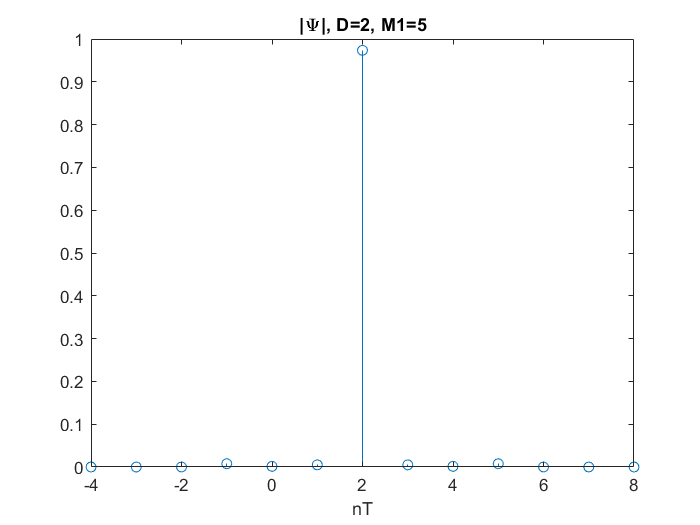
\includegraphics[width=\textwidth]{figs/A_psi.png} 
		\caption{Magnitude of the impulse response of the system $\psi$ in point A.}
		\label{fig:A_psi}
	\end{center}
\end{figure}

The detected symbols $a_{k-D}$ are chosen using a threshold detector that analyzes the sign of the imaginary and real part of the input complex value. The same detector is also used at point B, C and D.


\section*{Point B}

For point B the system is the same as in point A up to the equalizer, so the choice of $\bar{t}_0=16$ (17 with Matlab indexing) is the same. The matched filter is the same as in point A, see figure \ref{fig:B_gm}. However in this case we equalize with a DFE, that is made of two filters called feedforward and feedback filter denoted by $c$ and $b$. The feedforward filter has the role of equalizing only the precursors of the overall impulse response, while the ISI due to postcursors will be canceled by filter $b$ positioned on a feedback loop between the output of the threshold detector and its input. 

\begin{figure}[H]
	\begin{center}   
		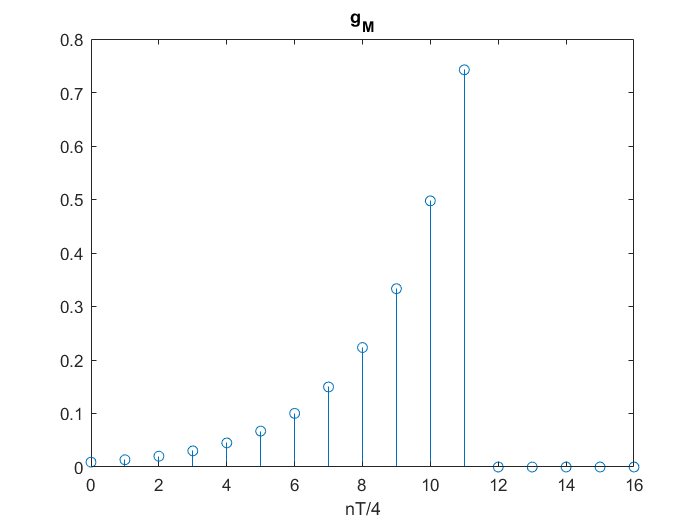
\includegraphics[width=\textwidth]{figs/B_gm.png} 
		\caption{Impulse response of the matched filter $g_{M}$ for the receiver in point B.}
		\label{fig:B_gm}
	\end{center}
\end{figure}

The computation of the optimal filters $c$ and $b$ is carried out using the Wiener filter approach. The relation between the input random process and the output is:
\begin{equation}
\begin{split}
y_k &= x_{FF,k} + x_{FB,k} \\
&= \sum_{i=0}^{M_1-1}c_ix_{k-i} + \sum_{j=1}^{M_2}b_ja_{k-D-j}
\end{split} 
\end{equation}
where $M_1$ is the order of the feedforward filter, $M_2$ is the order of the feedback filter and $a_{k-D}$ are the already detected past symbols fed back through $b$. Defining postcursors and precursors as in point A, we have that we can apply the Wiener-Hopf equations on the process:
\begin{equation} \label{eq:yk}
y_k = \sum_{i=0}^{M_1-1}c_i \left(x_{k-i}-\sum_{j=1}^{M_2}h_{j+D-i}a_{k-j-D} \right)
\end{equation}

The result can be easily computed as $c_{opt} = \vt{R}^{-1}\vt{p}$ once we find the autocorrelation matrix $\vt{R}$ and the correlation vector $\vt{p}$, expressed as \cite{nevio<3}:

\begin{equation} \label{eq:wienerR}
\mathbf{[R]}_{p,q} = \sigma_a^2 \left( \sum_{j=-N_1}^{N_2}h_jh^*_{j-(p-q)}-\sum_{j=1}^{M_2}h_{j+D-q}h^*_{j+d-p} \right) + r_{\tilde{w}}(p-q)
\end{equation}
\begin{equation} \label{eq:wienerp}
\mathbf{[p]}_p = \sigma_a^2 h^*_{D-p} \quad\quad\quad\quad\quad\quad p = 0,1,\dots,M_1-1
\end{equation}

where for a QPSK scheme $\sigma_a^2=2$ because it is the sum of two orthogonal components each with power $1$. The values of $r_{\tilde{w}}$ are the result of the autocorrelation of the noise after being filtered by $g_M$, so being the noise white we have $r_{\tilde{w}}(n)=N_0r_{g_M}(nT)$. At this point we can define the overall impulse response up to the threshold detector $\psi = h*c_{opt}$ and derive the optimal coefficients for filter $b$ as $b_i=-\psi_{i+D}$ for $i=1,\dots,M_2$.

The value of the cost function $J_{min}$ obtained using these the optimal filters is :
\begin{equation} \label{eq:jmin}
J_{min} = \sigma^2_a \left( 1-\sum_{l=0}^{M_1-1} c_{opt,l}h_{D-l}\right)
\end{equation}

Again the parameters to choose are the order of filter $c$, $M_1$, and the delay introduced $D$. This is because the order of $b$ can be chosen in such a way that all the postcursors are canceled by the feedback: $M_2=N_2+M_1-D-1$, and also the expression of the autocorrelation matrix significantly simplifies. The choice is carried out by selecting the values that minimize the functional $J_{min}$, this time being $M_1=5$ and $D=4$, and consequently $M_2=4$ because $N_2=4$. In figure \ref{fig:B_c}, \ref{fig:B_psi} and \ref{fig:B_b} we plot the resulting filters $c$, $\psi$ and $b$ at sampling time $T$. 

\begin{figure}[H]
	\begin{center}   
		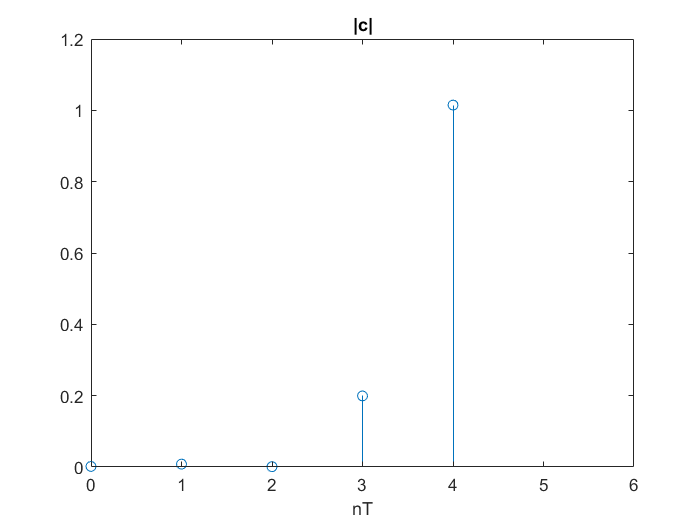
\includegraphics[width=\textwidth]{figs/B_c.png} 
		\caption{Magnitude of the impulse response of the filter $c$ (feedforward filter) for the receiver in point B.}
		\label{fig:B_c}
	\end{center}
\end{figure}

\begin{figure}[H]
	\begin{center}   
		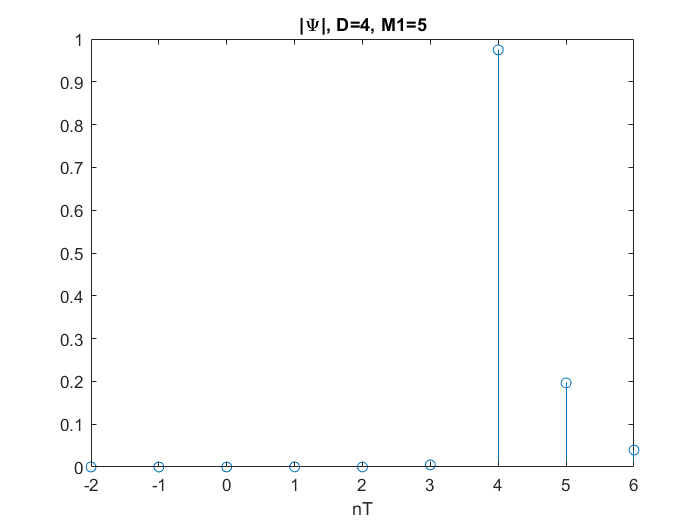
\includegraphics[width=\textwidth]{figs/B_psi.png} 
		\caption{Magnitude of the impulse response of the system $\psi$ in point B.}
		\label{fig:B_psi}
	\end{center}
\end{figure}

\begin{figure}[H]
	\begin{center}   
		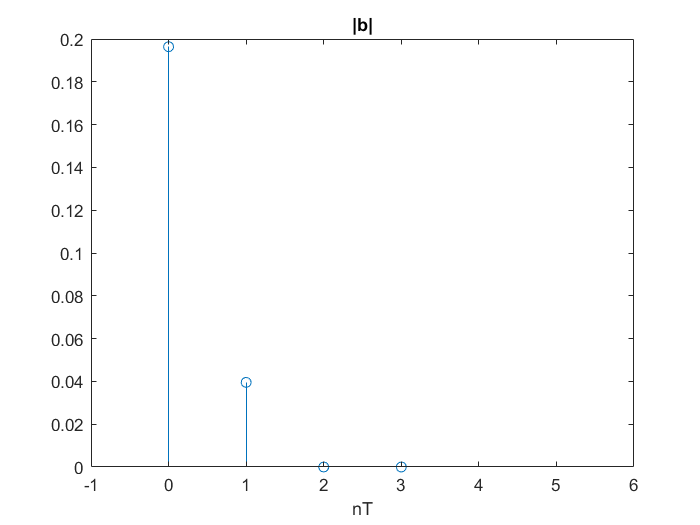
\includegraphics[width=\textwidth]{figs/B_b.png} 
		\caption{Magnitude of the impulse response of the filter $b$ (feedback filter) in point B.}
		\label{fig:B_b}
	\end{center}
\end{figure}


\section*{Point C}

In the receiver at point C we use a different type of approach. Before sampling the received signal we use an anti-aliasing filter instead of a matched filter. This is not an optimal solution but can be useful in some situation where the channel is not known or varies in time. Also the downsampling is at $T/2$ instead of $T$ and this gives more degrees of freedom in the equalization and more robustness with respect to the choice of the timing phase. The anti-aliasing filter has to avoid overlapping in frequency when we downsample the signal at the output of the channel. Our signal has frequency content that is periodic of period $4/T$, and has the shape of $|Q_c|^2$. Therefore its bandwidth is not limited and our anti-aliasing filter $g_{AA}$ will remove useful information because we cannot apply the Shannon theorem. The sampling at $T/2$ causes the frequency content of the signal to be repeated every $2/T$, causing an overlap. To avoid this, the cutting frequency of $g_{AA}$ has to be around $1/T$. In figure \ref{fig:C_gaa} we show the magnitude of the frequency response $|G_{AA}|$, where we chose the passband at $0.45 \cdot 2/T$ and the stopband at $0.55\cdot 2/T$.

\begin{figure}[H]
	\begin{center}   
		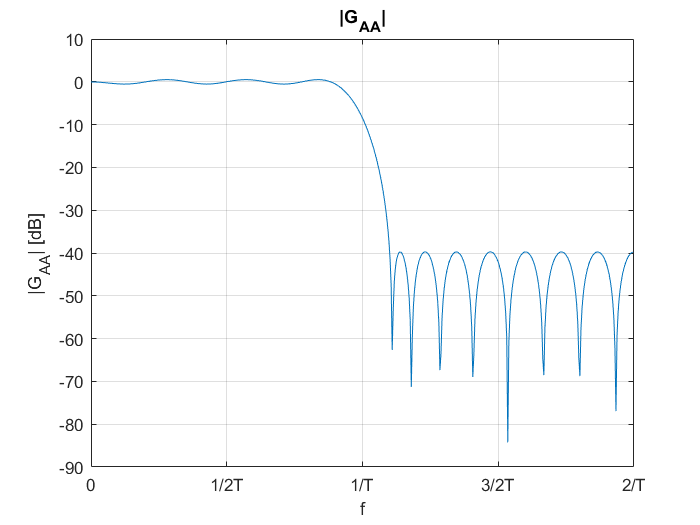
\includegraphics[width=\textwidth]{figs/GAA.png} 
		\caption{Magnitude of the frequency response of the anti-aliasing filter in point C.}
		\label{fig:C_gaa}
	\end{center}
\end{figure}

\begin{figure}[H]
	\begin{center}   
		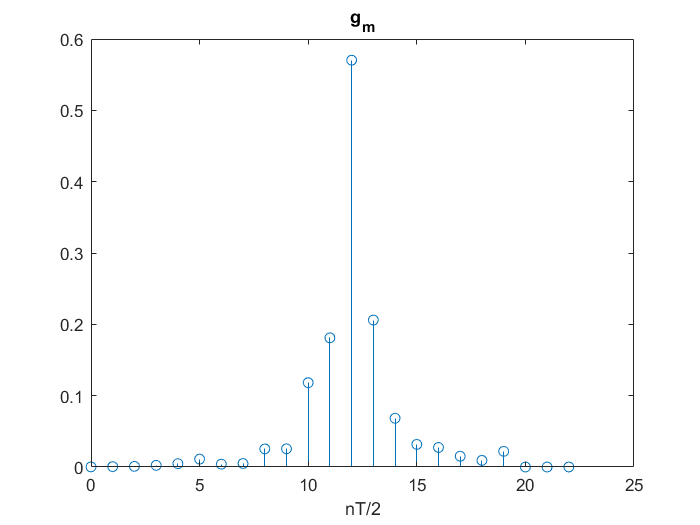
\includegraphics[width=\textwidth]{figs/C_gm.png} 
		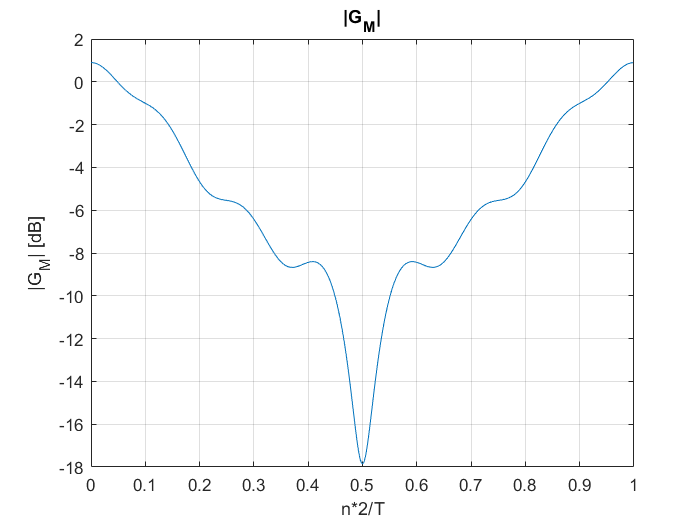
\includegraphics[width=\textwidth]{figs/GM_CD.png}
		\caption{Impulse and frequency response of the matched filter in point C.}
		\label{fig:C_gm}
	\end{center}
\end{figure}

The sampling then has to start after an offset $\bar{t}_0$ equal to the peak of the overall impulse response $q_c*g_{AA}$ at time $T/4$ that in this case was equal to $20$ (21 with Matlab indexing).  
In this kind of configuration we also add a digital matched filter after the sampling that is different from the previous points, now the matched filter is given by flipping and taking the conjugate of the whole impulse response $q_c*g_{AA}$ at sampling time $T/2$:
\begin{equation}
g_M = \left\{ q_c * g_{AA} \right\}^* \left(t_0 + i \frac{T}{2}\right) 
\end{equation}
The impulse response and frequency response are depicted in figure \ref{fig:C_gm}. 
In this case we use again a DFE. To derive the coefficients of the equalizer. Now the $c$ filter works at $T/2$ so the equations used for the Wiener solution aren't the same used for the points A and B. The equations \ref{eq:yk}, \ref{eq:wienerR} and \ref{eq:wienerp} become
\begin{equation} \label{eq:C_yk}
y_k = \sum_{i=0}^{M_1-1}c_i \left(x_{2k-i}-\sum_{j=1}^{M_2}h_{2(j+D)-i}a_{k-j-D} \right)
\end{equation}
\begin{equation} \label{eq:C_wienerR}
\mathbf{[R]}_{p,q}  = \sigma_a^2 \left( \sum_{n=-\infty}^{\infty}h_{2n-q}h^*_{2n-p}-\sum_{j=1}^{M_2}h_{2(j+D)-q}h^*_{2(j+D)-p} \right) + r_{\tilde{w}}(p-q) \\
\end{equation}
\begin{equation} \label{eq:C_wienerp}
\mathbf{[p]}_p = \sigma_a^2 h^*_{2D-p} \quad\quad\quad\quad\quad\quad p,q = 0,1,\dots,M_1-1
\end{equation}

where for a QPSK scheme $\sigma_a^2=2$ because it is the sum of two orthogonal components each with power $1$. The values of $r_{\tilde{w}}$ are the result of the autocorrelation of the noise after being filtered by $g_{AA}$ and $g_M$, so being the noise white we have $r_{\tilde{w}}(n)=N_0r_{g_M * g_{AA}}(nT/2)$. It is important to note that the matrix $\vt{R}$ obtained is ill conditioned because of the reduced sampling time $T/2$. To solve this problem we added a small constant along the diagonal of $\vt{R}$ to increase its determinant while not altering too much the solution of the linear system.

 At this point we can define the overall impulse response up to the threshold detector $\psi = h*c_{opt}$ and derive the optimal coefficients for filter $b$ as $b_i=-\psi_{2(i+D)}$ for $i=1,\dots,M_2$ because filter $b$ works at $T$. 

The value of the cost function $J_{min}$ obtained using these the optimal filters is :
\begin{equation} \label{eq:C_jmin}
J_{min} = \sigma^2_a \left( 1-\sum_{l=0}^{M_1-1} c_{opt,l}h_{2D-l}\right)
\end{equation}

Again the parameters to choose are the order of filter $c$, $M_1$, and the delay introduced $D$. This is because the order of $b$ can be chosen in such a way that all the postcursors are canceled by the feedback: $M_2=N_2+M_1-D-1$, and also the expression of the autocorrelation matrix significantly simplifies. The choice is carried out by selecting the values that minimize the functional $J_{min}$, this time being $M_1=9$ and $D=4$, and consequently $M2=23$ because $N_1=N_2=19$  In figure \ref{fig:C_c}, \ref{fig:C_psi} and \ref{fig:C_b} we plot the resulting filters $c$, $\psi$ at sampling time $T/2$ and $b$ at sampling time $T$. In the fractionally spaced version of the DFE the aim is again to obtain an overall pulse $\psi$ that satisfies the Nyquist conditions at time $T$ so the samples at even multiples of $T/2$ are not used in the equalizer and are therefore a degree of freedom of the system.

\begin{figure}[H]
	\begin{center}   
		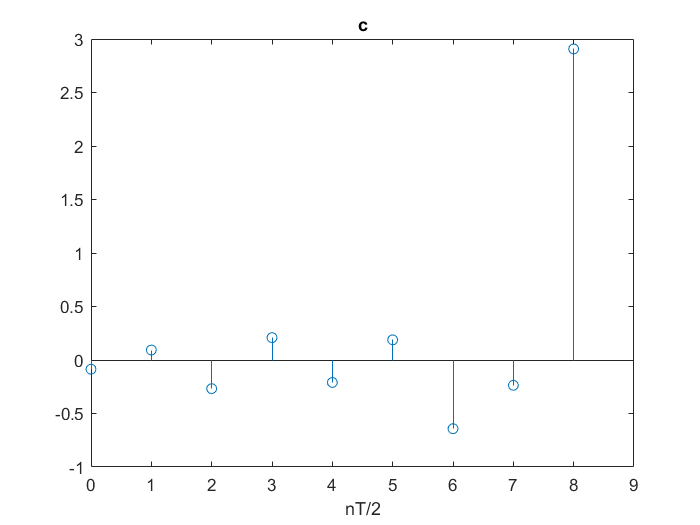
\includegraphics[width=\textwidth]{figs/C_c.png} 
		\caption{Magnitude of the impulse response of the filter $c$ (feedforward filter) for the receiver in point C.}
		\label{fig:C_c}
	\end{center}
\end{figure}

\begin{figure}[H]
	\begin{center}   
		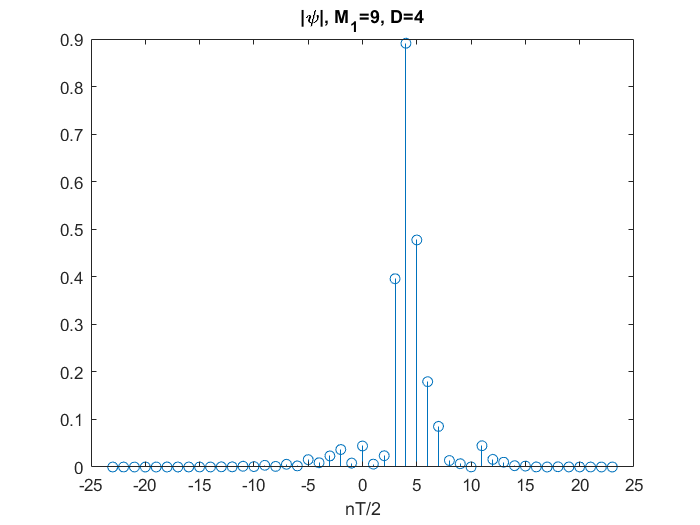
\includegraphics[width=\textwidth]{figs/C_psi.png} 
		\caption{Magnitude of the impulse response of the system $\psi$ in point C.}
		\label{fig:C_psi}
	\end{center}
\end{figure}

\begin{figure}[H]
	\begin{center}   
		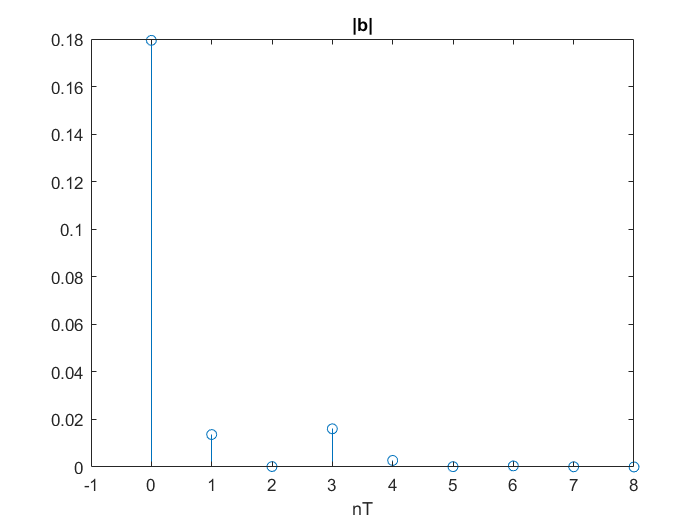
\includegraphics[width=\textwidth]{figs/C_b.png} 
		\caption{Magnitude of the impulse response of the filter $b$ (feedback filter) in point C.}
		\label{fig:C_b}
	\end{center}
\end{figure}

\section*{Point D} 

In this configuration the setup is similar to point C but without the matched filter after the downsampling at $T/2$. This means that all the burden of equalization and reduction of the noise is on filter $c$. The parameter $\bar{t}_0$ is 20 as before (21 with Matlab indexing), because the impulse response of the anti-aliasing filter and of $q_c$ have not changed. The equations for the derivation of the DFE filters with a Wiener approach are \ref{eq:C_wienerR} and \ref{eq:C_wienerp} and the parameters, chosen again by minimizing the value of $J_{min}$ are $M_1=9$, $D=4$ and consequently $M_2=N_2+M_1-D-1=16$ because this time $h$ is not symmetric and $N_2=12$. In figure \ref{fig:D_c}, \ref{fig:D_psi} and \ref{fig:D_b} we show the magnitude of the coefficients of filter $c$, $\psi$ and $b$.

\begin{figure}[H]
	\begin{center}   
		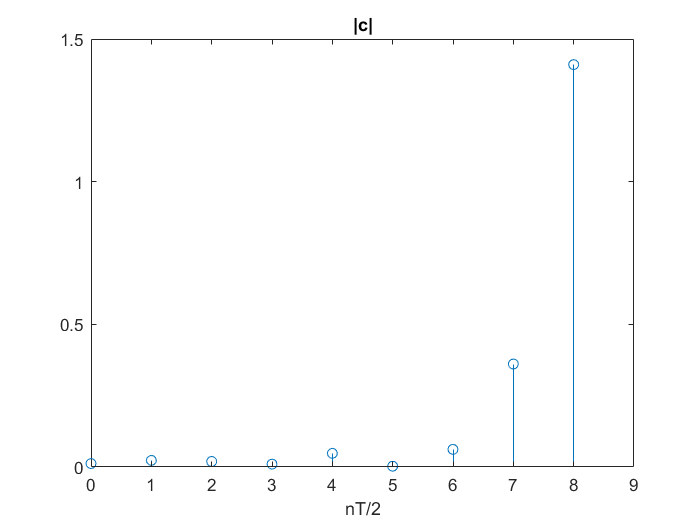
\includegraphics[width=\textwidth]{figs/D_c.png} 
		\caption{Magnitude of the impulse response of the filter $c$ (feedforward filter) for the receiver in point D.}
		\label{fig:D_c}
	\end{center}
\end{figure}

\begin{figure}[H]
	\begin{center}   
		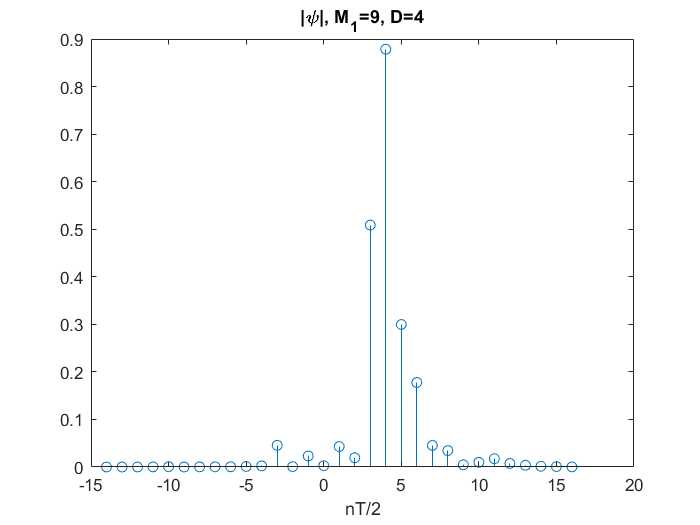
\includegraphics[width=\textwidth]{figs/D_psi.png} 
		\caption{Magnitude of the impulse response of the system $\psi$ in point D.}
		\label{fig:D_psi}
	\end{center}
\end{figure}

\begin{figure}[H]
	\begin{center}   
		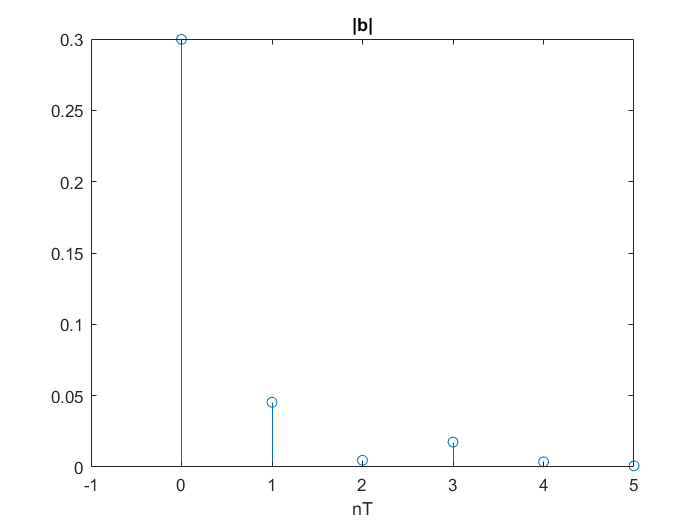
\includegraphics[width=\textwidth]{figs/D_b.png} 
		\caption{Magnitude of the impulse response of the filter $b$ (feedback filter) in point D.}
		\label{fig:D_b}
	\end{center}
\end{figure}

The following table sums up the final parameters for the 4 configurations A, B, C, D.

\begin{table}[htbp]
	\begin{center}
		\begin{tabular}{p{2.7cm}cccccc}
			\toprule
			& \multicolumn{2}{c}{Length of $h$} & \multicolumn{4}{c}{Parameters} \\
			\cmidrule(lr){2-3}
			\cmidrule(lr){4-7}
			Point & $N_1$ & $N_2$ & $M_1$ & $M_2$ & $D$ & $\bar{t}_0$ \\
			\midrule
			A &  4  &  4  & 5 & 0  & 2 & 16 \\
			B &  4  &  4  & 5 & 4  & 4 & 16 \\
			C & 19  &  19 & 9 & 23 & 4 & 20 \\
			D & 10  &  12 & 9 & 16 & 4 & 20 \\
			\bottomrule
		\end{tabular}
	\end{center}
	\label{tab:sumup}
	\caption{Choices for the various parameters in the different receiver implementations with respect to the length of $h$.}
\end{table} 

\section*{Point E}

In this point we use the Viterbi algorithm (VA) to implement the Maximum Likelihood criterion for data detection. 
For the execution of the algorithm we consider the signal $y_k$ at the output of filter $c$ in the schema at point B:
\begin{equation}
y_k = \psi_D a_{k-D} + \psi_{D+1} a_{k-D-1} + \dots +\psi_{D+M_2} a_{k-D-M_2} + w_k
\end{equation}
where $w_k$ includes the residual ISI and the noise. The useful signal $u_k$ can then be taken as $u_k=\psi_D a_{k-D} + \psi_{D+1} a_{k-D-1} + \dots +\psi_{D+M_2} a_{k-D-M_2}$ and if we call $y_k=z_k$ we have the usual setup for VA: $z_k = u_k+w_k$. We will have then that the number of states is $N_s=M^{M_2}$ where $M$ is 4, the cardinality of the QPSK constellation. In the specific case of point B $M_2=4$ so $N_s=256$. We define the state basing ourselves of the choice of $u_k$ so:
\begin{equation}
\begin{split}
\vt{s}_k = \{a_{k-D}, a_{k-D-1}, a_{k-D-2}, \dots, a_{k-(M_2-1)}\} = \\
= \{a_{k-D}, a_{k-D-1}, a_{k-D-2}, a_{k-D-3}\}
\end{split}
\end{equation}

\section*{Point F}

Here we apply the forward-backward algorithm to implement the MAP criterion for detection. Actually, we use an approximation of the algorithm called max-log MAP that is computationally more simple. The state definition we used is the same as in point E, due to the fact that the system is the same up to the decision point:
\begin{equation}
u_k=\psi_D a_{k-D} + \psi_{D+1} a_{k-D-1} + \dots +\psi_{D+M_2} a_{k-D-M_2}
\end{equation}
and
\begin{equation}
\begin{split}
\vt{s}_k = \{a_{k-D}, a_{k-D-1}, a_{k-D-2}, \dots, a_{k-(M_2-1)}\} = \\
= \{a_{k-D}, a_{k-D-1}, a_{k-D-2}, a_{k-D-3}\}
\end{split}
\end{equation}
Again the number of states is $N_s=M^{M_2}$.




\section*{Simulation results}

The simulation of the six different receivers has been carried out using as input the result of applying a QPSK bitmap on a PN sequence with $r=20$ and length $L=2^r-1$. The length of the resulting input in terms of symbols is $524287$, because each symbol requires 2 bits to be determined. The obtained symbols are assumed to be distributed approximately as random. Given that we have to estimate the probability of error over 7 different values of the SNR (from 8 dB to 14 dB) for a range of values going from $10^{-1}$ to $10^{-4}$, we need to be sure that our estimate is not affected by a high variance. The estimator we chose is:
\begin{equation}
\hat{P}_e = \frac{\#_{wrong}}{\#_{tx}}
\end{equation}
where $\#_{wrong}$ is the number of erroneously detected symbols and $\#_{tx}$ is the total number of transmitted symbols. As $\#_{tx}$ increases the estimator becomes approximately a Gaussian random variable, unbiased and with variance: $\frac{P_e (1-P_e)}{\#_{tx}}$. This confirms that our estimate is reliable because the resulting variance will be very small, according to the empirical rule for which if we want to estimate a $P_e$ of $10^{-k}$, we need to measure it transmitting at least $30\cdot 10^{k}$ symbols. Indeed in our case the smallest $P_e$ we need to estimate is $10^{-4}$ and so the required number of symbols would be $30\cdot 10^{4}= 300000$ that is much less than our $\#_{tx}=524287$.

The results obtained are showed in figure \ref{fig:SNR}. In green we plotted the values of the $P_e$ according to the matched filter bound, as in the theoretical formula and from simulation\footnote{To simulate the matched filter bound we gave as input of a threshold detector the QPSK symbols $a_k$ disturbed only by noise, so neglecting the effect os ISI as we would have with an ideal non dispersive channel.}. In blue we have the LE (solid) and DFE (dashed) of points A and B. Their performance is very good, as we could guess by seeing the result of the overall pulse $\psi$ (see figure \ref{fig:A_psi} and \ref{fig:B_psi}, the ISI is almost completely canceled in both cases).
In case of receivers C and D (black dashed and black solid lines) the performances are worse, because the anti aliasing filter cuts a component of the useful signal and causes a permanent loss of information. Nevertheless the result is acceptable and could be considered as an alternative in those cases where a matched filter is not available or impracticable. The best results are achieved as expected by the Viterbi and forward-backward algorithms, that yield values of the $P_e$ almost equal to those of the bound. These performances however come at the cost of a higher computational load, indeed the 2 algorithms are significantly slower than the LE and DFE and require more memory.


\begin{figure}[H]
	\begin{center}   
		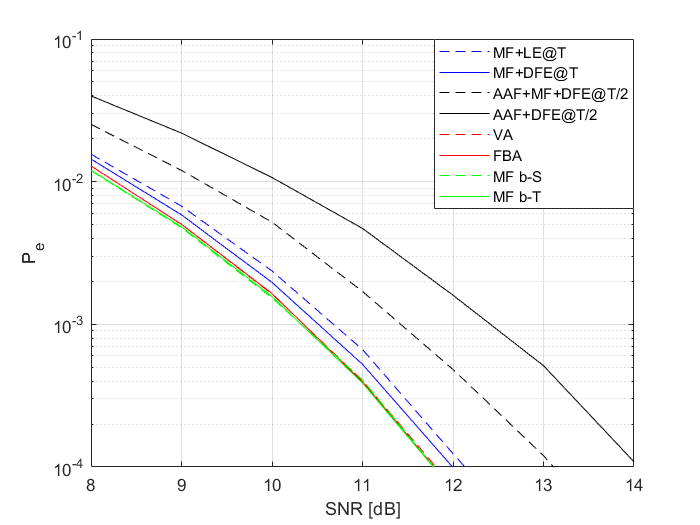
\includegraphics[width=\textwidth]{figs/SNR_Pe.png} 
		\caption{Results of the simulation over values of the SNR at the channel output from 8 dB to 14 dB.}
		\label{fig:SNR}
	\end{center}
\end{figure}


 
\begin{thebibliography}{15}
	
	\bibitem{nevio<3}
	Nevio Benvenuto, Giovanni Cherubini,
	\textit{Algorithms for Communication Systems and their Applications}. 
	Wiley, 2002.
	

	
\end{thebibliography}

\end{document}